\documentclass[pra,superscriptaddress,groupedaddress,twocolumn]{revtex4}
\usepackage{graphicx}  % needed for figures
\usepackage{dcolumn}   % needed for some tables
\usepackage{bm}        % for math
\usepackage{amssymb,amsmath} % for math
\usepackage{tikz} % for drawing
%\usepackage{subfig} % for subfigure
\usetikzlibrary{calc} % for tikz calculations
\usetikzlibrary{arrows,decorations.markings} % make arrow head bigger
\usepackage{array} % for changing table height
\usepackage{comment}
\usepackage[bookmarks]{hyperref}
\usepackage{threeparttable}
%\usepackage{siunitx} % for decimal alignment in tables
%\usepackage{arydshln} % for dashed line in tables

% avoids incorrect hyphenation, added Nov/08 by SSR
\hyphenation{ALPGEN}
\hyphenation{EVTGEN}
\hyphenation{PYTHIA}

\begin{document}

\title{Accurate predictions of ionization and atomization energies without the Born-Oppenheimer approximation}
\author{Yubo Yang}
\affiliation{Department of Physics, University of Illinois, Urbana, Illinois 61801 USA}
\author{Ilkka Kyl\"{a}np\"{a}\"{a}}
\affiliation{Department of Physics, Tampere University of Technology, P.O.~Box 692, FI-33101 Tampere, Finland}
\affiliation{Department of Physics, University of Illinois, Urbana, Illinois 61801 USA}
\author{Norm M. Tubman}
\affiliation{Department of Physics, University of Illinois, Urbana, Illinois 61801 USA}
\author{Jaron T. Krogel}
\affiliation{Materials Science \& Technology Division, Oak Ridge National Laboratory, Oak Ridge, TN 37831}
%\author{Michael V. Pak}
%\affiliation{Department of Chemistry, University of Illinois, Urbana, Illinois 61801 USA}
\author{Sharon Hammes-Schiffer}
\affiliation{Department of Chemistry, University of Illinois, Urbana, Illinois 61801 USA}
\author{David M. Ceperley}
\affiliation{Department of Physics, University of Illinois, Urbana, Illinois 61801 USA}
\date{\today}


\begin{abstract}
In this work we calculate the non-relativistic ground-state energies of atomic and molecular systems both with and without the Born Oppenheimer approximation. For this we utilize the fixed-node diffusion Monte carlo method, in which the nodes depend both on the electronic and ionic positions. We report ground state energies, ionization energies and atomization energies to an accuracy of $0.1-3.0$mHa. We find the ionization energies of the atoms to be independent of the adiabatic assumption, showing that the coupling between the nucleus and valence electrons is not important in the ionization process. The atomization energies, however, are significantly influenced by the non-adiabatic coupling of electrons and nuclei. We demonstrate that the fixed node approximation provides a highly accurate and scalable approach to treating molecule systems beyond the Born Oppenheimer approximation. Moreover, further development of this approach is discussed by considering a multi-time-step scheme for moving the ions. 
\end{abstract}

\maketitle

\section{Introduction}
There has been several recent discoveries that suggest that quantum wave functions, which include both electronic and ionic degrees of freedom, have many interesting properties that have yet to be explored.  This includes the development of equations that exactly factorize a wave function into electron and ionic components~\cite{cederbaum1}, the disappearance of conical intersections in wave functions of model systems~\cite{gross2014}, and the use of quantum entanglement to study electronic and ionic density matrices~\cite{boent}.  Extending such studies to realistic systems is of broad interest and will considerably expand our understanding of electron-ion systems.   However, treatment of \textit{ab initio} electron-ion systems is challenging and applications have thus been limited.   The most accurate simulations of electron-ion wave functions are generally done with very specialized wave functions, which are limited to rather small systems sizes \cite{mitroy2013}.  

As a framework to address these problems in general realistic systems, we recently demonstrated that quantum Monte Carlo (QMC) can be combined with quantum chemistry techniques to generate electron-ion wave functions~\cite{Tubman_ECG}.  We treated realistic molecular systems and demonstrated that our method can be scaled to larger systems than previously considered while maintaing a highly accurate wave function.  In the following we extend our previous work by considering the simulation of a larger benchmark set of atoms and molecules.  We calculate ionization energies and dissociation energies which can be directly compared with previous benchmarking results.  We also consider using multiple time steps for different species in the imaginary time propagator, which is also developed and tested.  Additionally we consider other estimators and the errors associated by using a mixed estimator.

\section{Method}

\subsection{Fixed-Node Diffusion Monte Carlo (FN-DMC)}
Diffusion Monte Carlo is a projector method that evolves a trial wavefunction with a Hamiltonian in imaginary time and projects out the ground-state wavefunction.  For practical simulations of fermions, the fixed-node approximation is introduced, which depends only on set of electronic positions where a trial wave functions is equal to zero.  This approximation is different than approximations typically used in quantum chemistry calculations, and in this work we demonstrate that we can generate high quality nodal surfaces for full electron-ion wave functions. %in the infinite time limit. 
%The trial wavefunction is often produced by some other mean field method such as Hartree-Fock (HF) or Density Functional Theory (DFT). 
%Typically the fixed-node approximation is introduced to overcome the sign-problem suffered in fermion simulations. %due to the presence of nodes in the ground-state wavefunction. 
%FN-DMC is a powerful method, since its accuracy is only limited by the quality of the nodal surface of the trial wavefunction and the finite length of the calculation. 
%The uncertainty in the obtained ground-state energy is statistically controlled and may be shrunk arbitrarily by increasing computation time.
In the limiting case that  the trial wavefunction has the same nodal surface as the exact ground-state wavefunction, the final ground-state energy will be exact. Approximate nodal surface can be generated through optimization of the full wave function. Such approximate nodal surfaces have been tested and validated on a wide range of systems, and consistently provide an excellent approximation of the exact ground-state energy,  comparable to the state of the art in \textit{ab initio} simulations [{\bf refs.~here}].
 %albeit with rather large variance if the quality of the trial function is low. 
 In addition the energies generated with FN-DMC are variational with regards to the ground state energy.  %, that is, even when the nodes of the trial wavefunction are not exact the result will be a rigorous upper bound to the exact ground-state energy.

%With advances in wave function optimization, 
In all but a handful of previous QMC simulations,  ions are "clamped" to their equilibrium positions. Such an assumption is not fundamentally required by FN-DMC.  It is possible to optimize thousands of wave function parameters simultaneously with variational Monte Carlo ~\cite{Nightingale_Linear,Umrigar_Linear,Brown_Bench} .   In our previous work we found that the most important effect to optimize for were the nodes due to electron-electron correlations~\cite{Tubman_ECG}, and in this regard we use more sophisticated electronic terms in the wave function than the ion part of the wave function.  %the introduction of linear optimization method by Nightingale et. al.\cite{Nightingale_Linear} and Umrigar et. al.\cite{Umrigar_Linear},
% one can systematically improve the wave function ansatz generated by quantum chemistry calculations to obtain high quality wave functions for atoms and molecules as was done by Brown\cite{Brown_Bench} and Toulouse\cite{Toulouse_Bench}. 
%However, in these benchmark studies, the authors always worked within the adiabatic assumption, i.e., only the electronic Hamiltonian is used in evolving the trial wavefunction in imaginary time, while
  %Its inclusion is mostly due to a lack of mean field theories that include non-adiabatic effects. 
%Although there is significant effort in the quantum chemistry community to develop such methodology, until a standardized package is developed we will have to rely on modification of the QMC algorithm itself to include non-adiabatic effects. 
% To this end, we previously developed techniques to construct a high quality electron-ion wavefunction from standard quantum chemistry wave function.

\subsection{Electron Wavefunction and Optimization}
The are several different approaches for generating high quality wave functions ~\cite{Umrigar_Alleviation,Toulouse_Bench, Brown_Bench,Seth_Bench}. We use an initial guess for the wavefunction that is generated from complete active space self-consistent field (CASSCF) \cite{Chaban_MCSCF,Szabo} calculation using the quantum chemistry package GAMESS \cite{GAMESS}. The optimized orbitals are then used in a second order configuration interaction (SOCI) calculation to generate a series of configuration state functions (CSF)~\cite{Clark_Bench}. The multi-CSF expansion of the wavefunction  can be expressed in the following form,
\begin{align}
\Psi_{SOCI}(\vec{r})=\sum\limits_{i=1}^{N_{CSF}}\alpha_i\phi_i(\vec{r}), \label{eq:psi_gms}
\end{align}
where $\vec{r}$ refers to the spacial coordinates of all the electrons. $\phi_i(\vec{r})$ are the CSF generated from SOCI. We used the cc-pV5Z basis for all the atomic systems and Roos Augmented Triple Zeta ANO basis for molecular systems~\cite{dunning,roos}. %due to the limited ability to handle a large number of basis elements in GAMESS.

%A Jastrow factor $J(\vec{r},\vec{\beta})$, in the form of a B-spline with values $\vec{\beta}$ on a linear grid,
A Jastrow factor is then added to the wave function to correlate electron motion and smooth out the divergence in the local energy near the ions by imposing the cusp condition \cite{Kato}. Our Jastrow factor contains one and two body terms.  %electron-ion term, two electron-electron terms (one for same spin electrons, one for opposite spin electrons) and two electron-electron-ion terms. 
The full wave function being optimized is then
\begin{align}
\Psi_e(\vec{r})=e^{J(\vec{r},\vec{\beta})}\sum\limits_{i=1}^{N_{CSF}}\alpha_i\phi_i(\vec{r})\label{eq:psie}
\end{align}
We optimized the CSF and Jastrow coefficients $\vec{\alpha},\vec{\beta}$ simultaneously with QMCPACK \cite{QMCPACK}.

\subsection{Electron-Ion Wavefunction}

\begin{figure}[t]
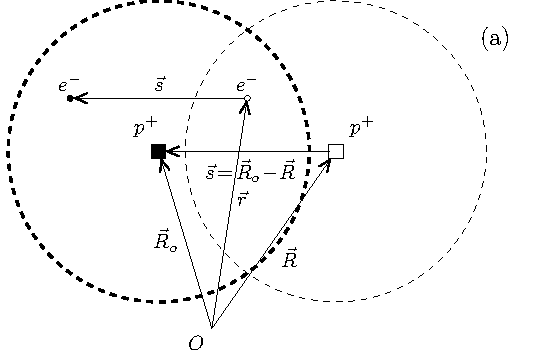
\includegraphics[width=9cm]{fig1a.pdf}
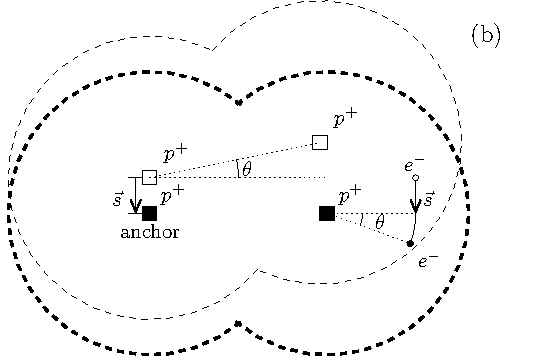
\includegraphics[width=9cm]{fig1b.pdf}
\caption{Dragged node approximation: {\bf (a)} For hydrogen atom, we assume the entire wavefunction shifts with the ion. This process can be visualized by following a contour of the wavefunction. The thick dashed circle represents a contour of the electron wavefunction when the proton is at its reference position $\vec{R}_o$ and the thin dashed circle represents the same contour when the proton has moved to a new position $\vec{R}$. To evaluate the ion-dependent electron wavefunction $\bar{\psi}_e(\vec{r},\vec{R})$, we simply map the electron to its proper place in the reference wavefunction $\psi_e(\vec{r})$. That is, $\bar{\psi}_e(\vec{r},\vec{R})=\bar{\psi}_e(\vec{r}+\vec{s},\vec{R}_o)=\psi_e(\vec{r}+\vec{s})$ where $\vec{s}$ is the shift required to put the proton back to its reference position. {\bf (b)} For H$_2^+$, we pick one of the protons as an "anchor" and approximate the new wavefunction by dragging the reference wavefunction with the "anchor" proton. We also rotate the wavefunction to align its axis of symmetry with the orientation of the two protons. \label{fig:drag}}
\end{figure}

Once a satisfactory electronic wave function has been obtained, we construct the electron-ion wave function using the ansatz we previously investigated~\cite{Tubman_ECG},
\begin{align}
\Psi_{ei}(\vec{r},\vec{R})=\psi_I(\vec{R})\bar{\psi}_e(\vec{r},\vec{R}), \label{eq:psi}
\end{align}
where $\vec{R}$ includes spatial coordinates of all ions. The ion wave function consists of simple products of Gaussian wave functions over each nuclei pair,
\begin{align}
\psi_I(\vec{R})\propto \prod\limits_{i,i<j}e^{-a(\vert \vec{R}-\vec{R}_j\vert-b_{ij})^2},
\label{wfs_ions}
\end{align}
where $a$ is a contraction coefficient for the ion wave function that we optimize for each system and $b_{ij}$ are taken to be the equilibrium distances between the nuclei at the minimum of the potential energy surface of the clamped nuclei. %Notice the new electron wavefunction $\bar{\psi}_e$ depends on both the electron and the ion positions. In general $\bar{\psi}_e(\vec{r},\vec{R})\neq\psi_e(\vec{r})$, but we do have $\bar{\psi}_e(\vec{r},\vec{R}_o)=\psi_e(\vec{r})$, where $\vec{R}_o$ are the ion positions used in the creation of the $\psi_e(\vec{r})$. The most straight-forward way to obtain $\bar{\psi}(\vec{r},\vec{R})$ is to repeat the process described in the previous section for every new ion positions $\vec{R}$. However, such an approach would be horrendously expensive. To alleviate the computational cost, Tubman {\it et al.}~proposed a "Dragged Node Approximation" \cite{Tubman_ECG}, where the contours (including the nodal surface) of $\psi_e(\vec{r})$ are dragged along the ions $\vec{R}$ to create $\bar{\psi}(\vec{r})$. 
In Fig.~\ref{fig:drag} we demonstrate this strategy for the simple cases of a hydrogen atom and a H$_2^+$ molecular ion. %For atoms, this "dragged-node" process is equivalent to re-running a quantum chemistry calculation and re-optimizing the wavefunction at each new ion position. However, for diatomic molecules, since the distance between ions fluctuates, the two processes will produce slightly different wavefunctions. It is also important to note that the trial wavefunction (\ref{eq:psi}) is still in Born-Oppenheimer form for each set of ion coordinates, that is we are essentially using the Born-Oppenheimer wavefunction as the starting point of FN-QMC. Nevertheless, without modifications to the Hamiltonian, FN-DMC will automatically include non-adiabatic effects not present in the trial wavefunction and the process remains variational.
Although the dragged-node technique is developed with atomic and diatomic systems in mind, it is not difficult to generalize it for use in larger systems or even apply to parts of a bigger system, e.g., treating light ions as quantum particles and heavy ions as "clamped". %For a system of more than 3 particles, a general fitting procedure \cite{Kabsch_Rotation} can be done to determine the transformation needed to put the ions back to their reference positions. This is similar to the process of protein structure alignment implemented in some well-known biophysics software such as VMD \cite{VMD}. Once the transformation is determined, we can map each electron individually and evaluate the wavefunction with moved ions using the reference wavefunction as was done for atoms and diatomics. One complication occurs when the ions become degenerate (when there are more than two protons with the same spin for example). In this case one has to explicitly anti-symmetrize the wavefunction of the ions, Eq.~\eqref{wfs_ions}, in a manner similar to what is done for the electron wavefunction (Slater determinant). 

\section{Results and Discussion}


\begin{table*}[t!]
\setlength{\extrarowheight}{1pt}
\begin{threeparttable}
\caption{Ground state energies for atoms and ions, and the ionization energies: Fixed-Node DMC results of this work (FN-DMC) for atoms and ions with and without the adiabatic assumption. The ionization potentials (IP) are reported in the last section of the table with the experimental values. Energies are given in units of Hartree. \label{tab:ionization}}
\begin{tabular*}{\textwidth}{@{\extracolsep{\fill}} cccccccccc}
\hline\hline
$\text{Atom}$ & $\text{Li}(^2\text{S)}$ & $\text{Be}(^1\text{S)}$ & $\text{B}(^2\text{P)}$ & $\text{C}(^3\text{P)}$ & $\text{N}(^4\text{S)}$ & $\text{O}(^3\text{P)}$ & $\text{F}(^2\text{P)}$ \\ \hline
&&&clamped nuclei&&&& \\
FN-DMC & $\text{-7.478056(4)}$ & $\text{-14.66732(1)}$ & $\text{-24.65377(1)}$ & $\text{-37.84449(2)}$ & $\text{-54.58858(3)}$ & $\text{-75.06576(4)}$ & $\text{-99.7316(1)}$ \\
Seth DMC \cite{Seth_Bench} & $\text{-7.478067(5)}$ & $\text{-14.667306(7)}$ & $\text{-24.65379(3)}$ & $\text{-37.84446(6)}$ & $\text{-54.58867(8)}$ & $\text{-75.0654(1)}$ & $\text{-99.7318(1)}$ \\
Davidson 1993 \cite{Davidson_Atoms} &  -7.47807 & -14.66736 & -24.65391 & -37.8450 &-54.5892 & -75.0673 & -99.7339 \\
&&&non-adiabatic&&&& \\
FN-DMC & $\text{-7.47742(1)}$ & $\text{-14.66643(2)}$ & $\text{-24.65244(3)}$ & $\text{-37.84277(6)}$ & $\text{-54.58655(8)}$ & $\text{-75.0631(1)}$ & $\text{-99.7290(4)}$ \\
\hline
%\end{tabular} \\ 
%\begin{tabular}{*{1}{*{8}{c}}}
$\text{Ion}$ & $\text{Li}^+(^1\text{S)}$ & $\text{Be}^+(^2\text{S)}$ & $\text{B}^+(^1\text{S)}$ & $\text{C}^+(^2\text{P)}$ & $\text{N}^+(^3\text{P)}$ & $\text{O}^+(^4\text{S)}$ & $\text{F}^+(^3\text{P)}$ \\ \hline
&&&clamped nuclei&&&& \\
FN-DMC & $-7.279919(4)$ & $\text{-14.324753(6)}$ & $\text{-24.34884(1)}$ & $\text{-37.43075(2)}$ & $\text{-54.05376(3)}$ & $\text{-74.56588(4)}$ & $\text{-99.0913(1)}$ \\
Seth DMC \cite{Seth_Bench} & $\text{-7.279914(3)}$ & $\text{-14.324761(3)}$ & $\text{-24.34887(2)}$ & $\text{-37.43073(4)}$ & $\text{-54.05383(7)}$ & $\text{-74.56662(7)}$ & $\text{-99.0911(2)}$ \\
Davidson 1993\tnote{a} \cite{Davidson_Atoms} & -7.27999 & -14.3249 & -24.3489 & -37.4312 & -54.0552 & -74.5668 & -99.0937 \\
&&&non-adiabatic&&&& \\
FN-DMC & $\text{-7.2793(1)}$ & $\text{-14.32386(2)}$ & $\text{-24.34750(3)}$ & $\text{-37.42904(4)}$ & $\text{-54.05182(9)}$ & $\text{-74.56336(8)}$ & $\text{-99.0885(3)}$ \\
\hline
&&&clamped nuclei&&&& \\
IP (FN-DMC) & 0.19814(1) & 0.34256(2) & 0.3049(3) & 0.4138(5) & 0.53475(8) & 0.500(1) & 0.640(1) \\
&&&non-adiabatic&&&& \\
IP (FN-DMC) & 0.1981(1) & 0.34257(2) & 0.3049(3) & 0.4137(5) & 0.53473(8) & 0.500(1) & 0.640(1) \\
IP (Exp.) \cite{Davidson_Atoms} & 0.19808 & 0.3425 & 0.30502 & 0.413797 & 0.533967 & 0.500526 & 0.640173 \\
\hline\hline
\end{tabular*}
\begin{tablenotes}
\item[a] The ionic ground state energies are calculated by adding ionization potentials in Table XII to the atomic ground state energies in Table XI from Ref.~\cite{Davidson_Atoms}.
\end{tablenotes}
\end{threeparttable}
\end{table*}

\subsection{Ground State Energies}

Ground state energies are calculated for first row atoms and ions with and without the adiabatic assumption, see Table \ref{tab:ionization}. %The first row of Table \ref{tab:ionization} lists the level of CASSCF calculation we used to generate the all-electron wavefunction guess. 
We first performed a CAS(m,n) calculation (m electrons into n active orbitals) with the ground-state equilibrium geometries taken from experimental data \cite{CCCBDB}. The MCSCF optimized orbitals are then used in a SOCI calculation that includes single and double excitations of the m electrons into all of the available valance orbitals provided by the basis. %The SOCI ground state CSF $\phi_0(\vec{r})$ always dominates the expansion (with $\alpha_0>0.95$). Nevertheless, 
We include all CSFs with coefficients bigger than some cutoff $\epsilon$ to lend reasonable flexibility to the wavefunction during optimization. %The choice of $\epsilon$ is somewhat arbitrary. 
We include as many CSFs as possible to maximize the flexibility of the wavefunction. However, the inclusion of too many CSFs with small expansion coefficients can introduces noise as they requires a large number of samples in the optimization step to be optimized. 
We have chosen to restrict the number of CSFs in the wave function to be $\sim$1000 in all systems. 
%to maintain a balance between the flexibility and the cost of optimization. In all of the atoms and molecules tested, this criteria results in an $\epsilon$ of $\sim 0.0001-0.001$, and the sum of coefficients squared of the included CSFs gives $\sum a_i^2 > 0.999$ in all cases. 
Optimization was performed with roughly $10^7$ statistically independent samples and we chose a cost function consisting of equal parts average local energy and reweighted variance. %We found this choice of cost function to produce slightly better wavefunctions than a highly biased one, albeit the differences are small and are most likely insignificant at the DMC level. 
  We performed timestep extrapolation for all of the tested systems. Five timesteps from $0.005~\text{Ha}^{-1}$ to $0.001~\text{Ha}^{-1}$ were used for all systems in the adiabatic FN-DMC.% smaller timestep ($0.0005~\text{Ha}^{-1}$) is used for systems with 7 or more electrons. %For such small timesteps almost all DMC runs have $>99\%$ acceptance rate, thus we expect the timestep error to be very small. Indeed, for systems with fewer than 7 electrons, the DMC energies at all tested timesteps agree within error bars, only larger systems exhibit linear extrapolation behavior.

The clamped nuclei ground state FN-DMC energies  are consistently equal across all systems, within error bars, with a recent QMC benchmark study~\cite{Seth_Bench}. This is an interesting coincidence since we used a different approach in optimizing our wave functions.   In particular our large multi-determinant expansions, can be compared with the approach used by Seth {\it et al.}~\cite{Seth_Bench} which used moderately-sized multi-determinant expansions ($\sim$ 100 CSF) with a backflow transformation.   %For example there is agreement to less than 0.2 mHa accuracy for F, when the actual ground state wave functions is known  
 %we both obtain almost the same DMC energies, but with very different wavefunctions.  
 For the atomic systems, there are two ECG calculations of non-adiabatic ground state energies we can use as benchmark.  The non-adiabatic ground-state energies for Be and B ($-14.66643(2)$~Ha and $-24.65244(3)$~Ha) are in agreement with ECG results  to an accuracy of less than 0.2 mHa (-$14.66643544$~Ha \cite{Bubin_BeH_noBO} and -$24.652598$~Ha~\cite{Bubin_BH_noBO}).  %The non-adiabatic energies for the rest of the atoms and their first ionization states in Table \ref{tab:ionization} have not been explicitly calculated.

We performed a study over diatomic systems, the results of which are presented in Table \ref{tab:atomization}. For these diatomic systems, there are semi-empirical benchmark results~\cite{Feller_Corrections}, for which we can compare our results againsts. %It is important to note that with our method, the only included non-adiabatic effects are the zero point motion of the nuclei and any correlation that may exist among the quantum particles. We do not take into account spin-orbit coupling or relativistic effects. 
%Therefore, we subtracted the corresponding corrections from the values of Ref.~\cite{Feller_Corrections}. 
To make the comparison against the semi-empirical results, we took the reference energies from the last column of Table VI of Ref.~\cite{Feller_Corrections} and subtracted the corrections in the $\Delta E_{SR}$ and SO columns for comparison with our non-adiabatic energies.  For the comparison with our adiabatic energies we subtracted the DBOC and ZPE corrections.  Corrections from spin-orbit coupling and relativistic effects are not used, as they are not included in our Hamiltonian.

%It should be emphasized that in principle our method is much simpler, since there is no need for separate computations for each correction factor, and thus, no addition of uncertainties. Further, the uncertainties in our calculations are statistically controlled and may be reduced by increasing computation time. 

\subsection{Ionization Energies}
The ionization energies are listed in Table \ref{tab:ionization} and they agree well with experimental results. Notice that even though ground state energies change significantly with the inclusion of non-adiabatic effects, the ionization energies match with or without the adiabatic assumption. This suggests that for atomic systems, coupling between valence electron and ion motions is small. The difference in ground state energies can be entirely attributed to the zero point motion of the nuclei. Physically, this means that for all first row atoms, the outer most electron is screened from the nucleus and all of the energy required for its removal can be attributed to its interaction with the rest of the electrons in the atom.

For the LiH molecule we are also interested in calculating the electron affinity for comparison to ECG results. We calculated the ground state energy of LiH$^-$ to be $-8.08220(2)$~Ha for the case of clamped nuclei.  With non-adiabatic effects included our result is  $-8.07811(3)$~Ha. Our non-adiabatic result is in good agreement with a previous ECG study \cite{Bubin_LiH_noBO} which reported a value of $-8.07856887$~Ha. We report an electron affinity of $0.01191(4)$~Ha which is can be compared to the ECG prediction of $0.012132(2)$~Ha and agrees with experiment $0.0126(4)$~Ha.  We note that $\text{LiH}$ ground state energies which we compare against are mislabeled in Ref.\cite{Bubin_LiH_noBO}, with $\text{LiH}^-$ and LiD being switched.% This also propagated to the following review paper~\cite{Mitroy_ECG}.


 
\subsection{Atomization Energies}
The ground state energies for various hydrides are reported in Table \ref{tab:atomization}. The energies calculated for clamped nuclei are on par with the best available quantum chemistry results \cite{Adamowicz_LiH,Koput_BeH,Miliordos_BH}. The energies calculated without the adiabatic assumption are in agreement with the ECG results for LiH, BeH to within 0.4 mHa.   In general for small systems, ECG results and typically orders of magnitude more accurate than the best QMC and quantum chemistry simulations.  However, with BH being one of the largest ECG simulations performed, the QMC results are actually lower in energy, in this case by 1 mHa.  For the systems CH, OH, and HF, there are no explicit simulations we can compare against, and we rely on the experimental results and the results with estimated non-adiabatic corrections for comparison.  Our biggest errors appear to occur for BeH and OH.   For the case of BeH our agree with accuracy higher than 1 mHa with both the ECG results and semi-empirical benchmarking.  In particular the ECG results are converged to more digits than the experimental error bar, and it is likely the experimental reference has errors on the order of 5 mHa.   For the case of OH, our error is on the order of 1 mHa, which isn't unexpected as our clamped nuclei ground state energy is roughly 3 mHa from the actual estimated ground state energy.%In the case of simple hydrides, non-adiabatic effects do make a noticeable contribution to the atomization energy. This is possibly due to the presence of the light weighted proton.
 
\begin{table*}[t!]
\setlength{\extrarowheight}{1pt}
\begin{threeparttable}
%\setlength{\extrarowheight}{3pt}
\caption{Ground state energies and atomization energies: Fixed-Node DMC results of this work for all first row hydrides with and without the adiabatic assumption. Energies are given in units of Hartree. \label{tab:atomization}}
\begin{tabular*}{\textwidth}{@{\extracolsep{\fill}} cccccccc}
\hline\hline
$\text{Molecule}$ & $\text{LiH }(^1\Sigma^+)$ & $\text{BeH }(^2\Sigma^+)$ & $\text{BH }(^1\Sigma^+)$ & $\text{CH }(^2\Pi)$ & $\text{OH }(^2\Pi)$ & $\text{HF }(^1\Sigma^+)$ \\ \hline
&&&clamped nuclei&&& \\
$E$ (this work) & $\text{-8.070521(7)}$ & $\text{-15.24793(1)}$ & $\text{-25.28868(2)}$ & $\text{-38.4781(1)}$ & $\text{-75.7352(1)}$ & $\text{-100.4556(2)}$ \\
$E_{\text{ref}}$ \tnote{a} \cite{Adamowicz_LiH,Koput_BeH,Miliordos_BH,Davidson_Atoms,Feller_Corrections} & $\text{-8.07045}$ & $\text{-15.247846}$ & $\text{-25.287650}$ & $\text{-38.4792(2)}$ & $\text{-75.7382(2)}$ & $\text{-100.4600(3)}$ \\
&&&non-adiabatic&&& \\
$E$ (this work) & $\text{-8.06620(2)}$ & $\text{-15.24196(7)}$ & $\text{-25.28103(4)}$ & $\text{-38.4704(4)}$ & $\text{-75.7237(4)}$ & $\text{-100.4445(5)}$ \\
ECG \cite{Bubin_LiH_noBO,Bubin_BeH_noBO,Bubin_BH_noBO} & $\text{-8.0664371(15)}$ & $\text{15.24203(10)}$ & $\text{-25.2803(10)}$ & $\text{N/A}$ & $\text{N/A}$ & $\text{N/A}$ \\
\hline
&&&clamped nuclei&&& \\
$D_{e}$ (this work) & 0.092465(8) & 0.08062(1) & 0.13491(2) & 0.13361(2) & 0.16944(4) & 0.2240(2) \\
Feller 2008\tnote{b} \cite{Feller_Corrections} & 0.09262(5) & 0.0809(4) & 0.1354(2) & 0.1342(2) & 0.1709(2) & 0.2258(3) \\
&&&non-adiabatic&&& \\
$D_{0}^0$ (this work) & 0.08905(2)  & 0.07580(7)  & 0.12886(5) & 0.1279(7) & 0.1610(4) & 0.2158(6) \\
Feller 2008\tnote{c} \cite{Feller_Corrections} & 0.08940(5) & 0.0761(4) & 0.1299(2) & 0.1276(2) & 0.1622(2) & 0.2166(3)\\
Exp. \cite{CCCBDB} & 0.08874(38) & 0.0826(11) & 0.1281(37) & 0.1275(5) & 0.1622(1) & 0.2158(3) \\
\hline\hline
\end{tabular*}
\begin{tablenotes}
\item[a] For the smaller systems (LiH, BeH and BH), ECG studies provide the best reference energies. For CH, OH and HF, we combined the atomic energies in Ref.~\cite{Davidson_Atoms} with the atomization energies in \cite{Feller_Corrections} to produce the reference energies.
\item[b] The non-relativistic atomization energy in the adiabatic limit are calculated by subtracting the scalar relativistic, spin-orbit coupling and zero-point energy corrections from the reference energies in Table VI of Ref.~\cite{Feller_Corrections}.
\item[c] Here only the scalar relativistic and spin-orbit coupling corrections are subtracted.
\end{tablenotes}
\end{threeparttable}
\end{table*} 


\section{Using multiple time-steps}
The results of this work given in Tables \ref{tab:ionization} and \ref{tab:atomization} were obtained from simulations where we moved the nuclei as often as the electrons, i.e., we have used the same time-step for each particle. However, we could also use different sized time-steps for each different particle species as long as they are, e.g., multiples of the smallest time-step. Due to the Trotter expansion \cite{lester1} this only affects the diffusion term in the diffusion Monte Carlo method, not the branching part. Thus, while applying the kinetic projection operator of the electrons for $M$ times with time-step $\tau$, a heavier particle can use a kinetic projector with time-step $\beta=M\tau$, which is applied only once. Our numerical tests with LiH molecule show that even with $M=1000$ for the proton, and $M=4000$ for the Li nucleus the results coincide with those shown in Table II, in which that nuclei were moved as often as the electrons. However, we believe that for the Li nucleus $M$ could be larger, since in the diffusion term the exponential has a prefactor of $m/2\tau$. Therefore, it is possible that $M$ could be roughly equal to the mass of the particle, since then the prefactor $m/2M\tau$ would roughly be equal to the one found accurate for the electrons.

The major benefit of this ''multi-time-stepping'' procedure is that going beyond the dragged-node approximation one needs to calculate on-the-fly updates for the electronic wave function each time the nuclei are moved. Thus, the possibility to make external program calls only every thousand steps in case of nonadiabatic hydrogen, and every four thousand (or even ten thousand) steps in case of Li nuclei will enable even more accurate calculations for more complex systems.


\section{Conclusion}
We calculated the ground-state energies of first row atoms and their corresponding ions and hydrides to an accuracy of $0.1$ mHa both with and without the adiabatic assumption. We found the ionization energies of the atoms to be independent of the adiabatic assumption, suggesting that either the energy difference between the adiabatic and non-adiabatic ground states is entirely due to the zero point motion of the nuclei or the coupling between the nucleus and electrons is not important in the ionization process. The atomization energies of simple hydrides, however, were significantly different in the adiabatic than in the non-adiabatic limit.  This is most likely due to the presence of the light nucleus, i.e.~the proton, in the molecule. We showed that it is necessary to include non-adiabatic effects to accurately predict the experimental values of atomization energies for these simple hydrides.

These calculations also verified the validity of the "dragged-node" approximation, namely it does indeed produce a high quality electron-ion trial wavefunction from a good electron wavefunction. This technique also has the potential to solve interesting larger-scale problems due to its ease of implementation as well as the polynomial scaling in computational time with respect to the number of electrons. As discussed the Method section, this technique can be generalized quite easily to deal with larger systems. In addition, we are able to offer similar levels of accuracy compared to the most sophisticated quantum chemistry methods (coupled cluster and ECG) while maintaining a reasonable level of computational and human cost.

\section{Acknowledgment}
This work was supported by the U.S. Department of Energy grant No. 1-485267-244000-191100 as part of the Scientific Discovery through Advanced Computing (SciDAC) program. We used the Extreme Science and Engineering Discovery Environment (XSEDE), which is supported by the National Science Foundation Grant No. OCI-1053575 and resources of the Oak Ridge Leadership Computing Facility (OLCF) at the Oak Ridge National Laboratory, which is supported by the Office of Science of the U.S. Department of Energy under Contract No. DE-AC05-00OR22725.


\bibliography{ref}
\end{document}
